\documentclass[12pt,twoside]{article}
\usepackage{amsmath, amssymb}
\usepackage{amsmath}
\usepackage[active]{srcltx}
\usepackage{amssymb}
\usepackage{amscd}
\usepackage{makeidx}
\usepackage{amsthm}
\usepackage{listings}
\usepackage{graphicx}
\usepackage{fixltx2e}
\usepackage{hyperref}
\usepackage{tikz, wasysym}
\usetikzlibrary{automata,positioning}
\renewcommand{\baselinestretch}{1}
\setcounter{page}{1}
\setlength{\textheight}{21.6cm}
\setlength{\textwidth}{14cm}
\setlength{\oddsidemargin}{1cm}
\setlength{\evensidemargin}{1cm}
\pagestyle{myheadings}
\thispagestyle{empty}
\markboth{\small{Pr\'actica 1. Eduardo, Daniel.}}{\small{.}}
\date{}
\begin{document}
\centerline{\bf An\'alisis de Algoritmos, Sem: 2020-1, 3CV2, Pr\'actica 1, 29 de enero de 2020}
\centerline{}
\centerline{}
\begin{center}
\Large{\textsc{Pr\'actica 1: Determinaci\'on experimental de la complejidad temporal de un
algoritmo}}
\end{center}
\centerline{}
\centerline{\bf {Mendoza Mart\'inez Eduardo, Aguilar Gonzalez Daniel.}}
\centerline{}
\centerline{Escuela Superior de C\'omputo}
\centerline{Instituto Polit\'ecnico Nacional, M\'exico}
\centerline{$edoomm8@gmail.com, daguilarglz97@gmail.com$}
\newtheorem{Theorem}{\quad Theorem}[section]
\newtheorem{Definition}[Theorem]{\quad Definition}
\newtheorem{Corollary}[Theorem]{\quad Corollary}
\newtheorem{Lemma}[Theorem]{\quad Lemma}
\newtheorem{Example}[Theorem]{\quad Example}
\bigskip
\textbf{Resumen:} La presente practica pretende mostrar el funcionamiento de dos algoritmos (suma binaria y mínimo común
divisor medieante el algoritmo de Euclídes) a través del tempo de ejecución.\\
{\bf Palabras Clave:} Algoritmo, Complejidad algorítmica, suma binaria, algoritmo de Euclides para mcd, tiempo de un algoritmo.
\section{Introducci\'on}
Los algoritmos están presentes en nuestra vida cotidiana y los usamos de manera inconsciente, ejemplo de esto 
es que los usamos para vestirnos, atarnos la agujetas, llegar a la escuela o trabajo, solucionar un problema
de cualquier \'indole, manual de usuario, etc.
As\'i como existen diferentes problemas de igual manera existen diferentes algoritmos de los cuales cada uno 
tiene diferente complejidad y tiempo de ejecución para llevarse a cabo. 
En esta practica se mostrará lo explicado ya que se implementan 2 algoritmos basicos una suma binaria de numeros 
de misma longitud y el llamado Algoritmo de Euclides con el cual se obtiene el maximo comun divisor de dos numeros. En
estos se prentende mostrar los diferentes tiempos de ejecuci\'on en que tardan cada uno y la utilizaci\'on de recursos
que requieren.
\section{Conceptos B\'asicos}
Para esta pr\'actica, se requiere conocer algunos conceptos básicos relacionados al análisis de los algoritmos, as\'i
como el funcionamiento de estos.

\subsection{Notación Theta}
La notación $ \Theta $ nos indica simultáneamente los límites
superior e inferior de ejecución, cuando estos están determinados
(en una misma función) por diferentes múltiplos reales positivos.\\
\\Es decir, t(n)$\epsilon \Theta(f(n))$ si y solo si t(n) pertenece
simultáneamente a $O$(f(n)) y a $\Omega$(f(n))
\\Expresado más formalmente decimos que $\Theta = (f(n)) = \Omega
(f(n) \cap O (f(n))$ . A esto también se le conoce como orden exacto
de f(n) ya que su tiempo de ejecución está acotado por arriba y por
abajo al mismo tiempo.

\subsection{Notación O}
Se dice que dada una función g(n), se define $O$(g(n)) como :
\\ \\$ O(g(n)) = \{f(n) | \exists n C_{1} \textgreater 0 y
n_{0} \textgreater 0 \amalg 0 \leq f(n) \leq C_{1}g(n)\} $

\subsection{Notación Omega Mayúscula}
Contrario a la notación O, la notación \(\Omega \) se usa para
determinar los límites inferiores en el consumo de recursos f(n)= \
(\Omega \) (g(n)) o lo que es lo mismo si existe una f( n ) \\
(\epsilon \Omega ( g ( n ) )\) constante real C\(>\)0 y una
constante entera $n_{0}$ \(\geq\)1 tal que f(n) \(\) Cg(n) para
cada entero n\(\geq\)\ $n_{0} $.
Aqu\'i va todo lo necesario para comprender el trabajo. En el caso de esta pr\'actica podr\'ian
colocar los conceptos de $\Theta$, $O$ y $\Omega$. Adem\'as comentar que algoritmos se
desarrollar\'an y mostrar los algoritmos, pueden mostrar ejemplos del funcionamiento del
algoritmo implementado.

\subsection{Algoritmo}
Serie de pasos bien definidos y finitos para resolver un problema.

\subsection{Suma binaria}
La suma o adición binaria es análoga a la de los números decimales. La diferencia radica en que en los números binarios se produce un acarreo (carry) cuando la suma excede de uno mientras en decimal se produce un acarreo cuando la suma excede de nueve(9). La suma binaria puede presentar las siguientes combinaciones:
\subsubsection{Combinaciones}
\begin{itemize}
\item 0 + 0 = 0
\item 0 + 1 = 1 
\item 1 + 0 = 1
\item 1 + 1 = 10
\end{itemize}
Note que al sumar 1 + 1 es  10, es decir, llevamos 1 a la siguiente posición de  la  izquierda  (acarreo).  Esto  es  equivalente,  en  el  sistema  decimal  a sumar  9  +  1,  que  da  10:  cero  en  la  posición  que  estamos  sumando  y  un 1 de acarreo a la siguiente posición.
\newline Los números o sumandos se suman en paralelo o en columnas, colocando un numero encima del otro. Todos los números bajo la misma columna tienen el mismo valor posicional.
\newline El orden de ubicación de los números no importa (propiedad conmutativa).

\subsection{Algoritmo de Euclides para mcd}
El algoritmo de Euclides es una técnica para encontrar rápidamente el MCD de dos enteros. El algoritmo es el siguiente:
\subsubsection{Combinaciones}
\begin{itemize}
\item Si A = 0 entonces MCD(A,B)=B, ya que el MCD(0,B)=B, y podemos detenernos.
\item Si B = 0 entonces MCD(A,B)=A, ya que el MCD(A,0)=A, y podemos detenernos. 
\item Escribe A en la forma cociente y residuo (A = B ⋅Q + R).
\item Encuentra MCD(B,R) al usar el algoritmo de Euclides, ya que MCD(A,B) = MCD(B,R).
\end{itemize}

\subsection{Complejidad Algor\'itmica}
La complejidad algorítmica representa la cantidad de recursos (temporales) que necesita un algoritmo para resolver un
problema y por tanto permite determinar la eficiencia de dicho algoritmo.

\section{Experimentaci\'on y Resultados}
\subsection{Suma binaria}
Para esta parte de la pr\'actica fue necesario implementar un algoritmo capaz de realizar una suma 
binaria entre dos t\'erminos A y B. El algoritmo se muestra a continuaci\'on en pseudoc\'odigo.
\begin{lstlisting}
suma (A[1, ..., n], B[1, ..., n])
  i <- n - 1
  acarreo <- 0
  C[n]

  while i != -1 do
	if acarreo == 0 then
	  if A[i] == 0 and B[i] == 0 then
	    acarreo <- 0
	    c <- 0
	  else if A[i] == 1 and B[i] == 1 then
	    acarreo <- 1
	    c <- 0
	  else
	    acarreo <- 0
	    c <- 1
	else
	  if A[i] == 0 and B[i] == 0 then
	    acarreo <- 0
	    c <- 1
	  else if A[i] == 1 and B[i] == 1 then
	    acarreo <- 1
	    c <- 1
	  else
	    acarreo <- 1
	    c <- 1

	C[0] <- c
	i <- i - 1

if acarreo == 1 then
  C[0] <- acarreo
\end{lstlisting}
Las pruebas de escritorio se implementaron en Python y a continuac\'on se muestran algunas pruebas con 
n\'umeros binarios aleatorios de n\'umero de bits no requeridos, esto con el fin de verificar si las sumas las 
hace correctamente.
\begin{center}
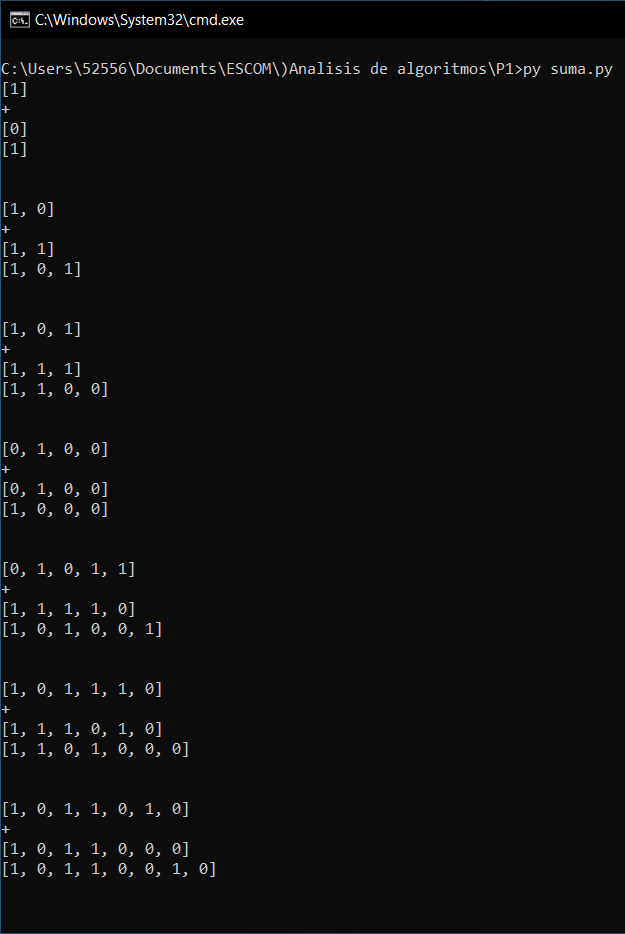
\includegraphics[height = 11cm]{suma}
\end{center}
Una vez verificado los resultados, procedimos a cambiar el n\'umero de bits a los acordados, es decir, a potencias 
de 2, y en vez de mostrar la suma, mostramos el tiempo de ejecuci\'on, como se muestra a continuaci\'on.
\begin{center}
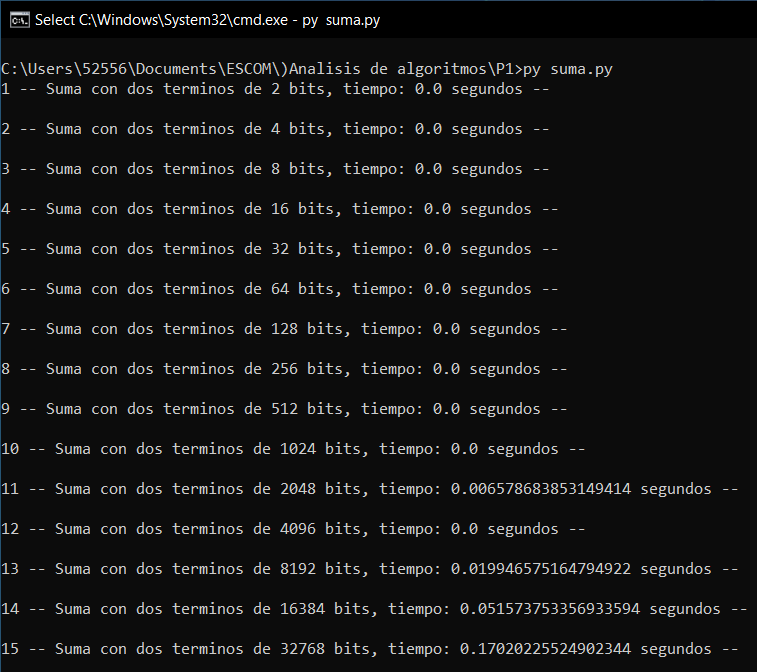
\includegraphics[height = 7.5cm]{tiempo}
\end{center} 
La gr\'afica de estos primeros tiempos quedo conformada de la siguiente forma
\begin{center}
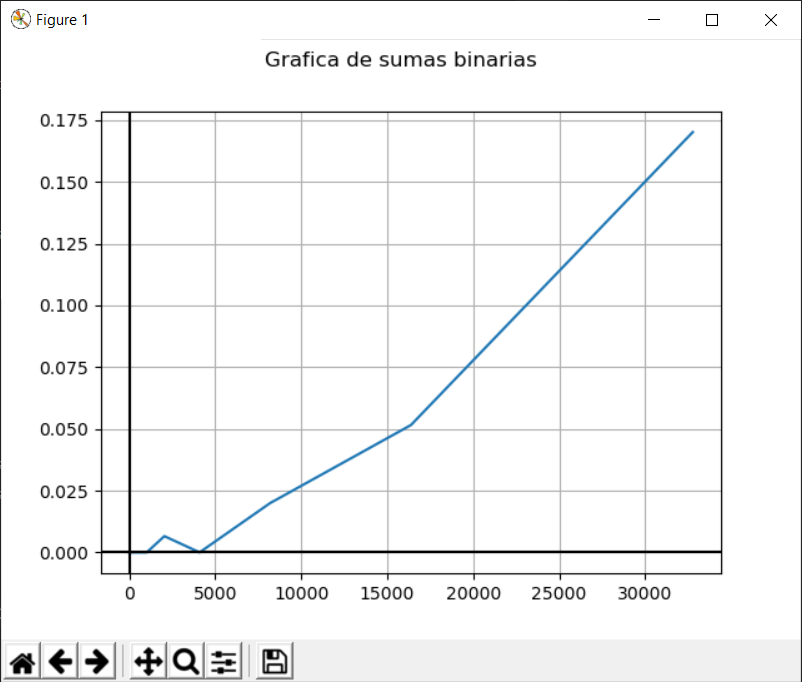
\includegraphics[height = 7.5cm]{g1}
\end{center}
Este mismo experimento se realizo incrementando el n\'umero de bits uno a uno, tal que fue posible observar la forma 
de la curva que va tomando el algoritmo implementado.
\begin{center}
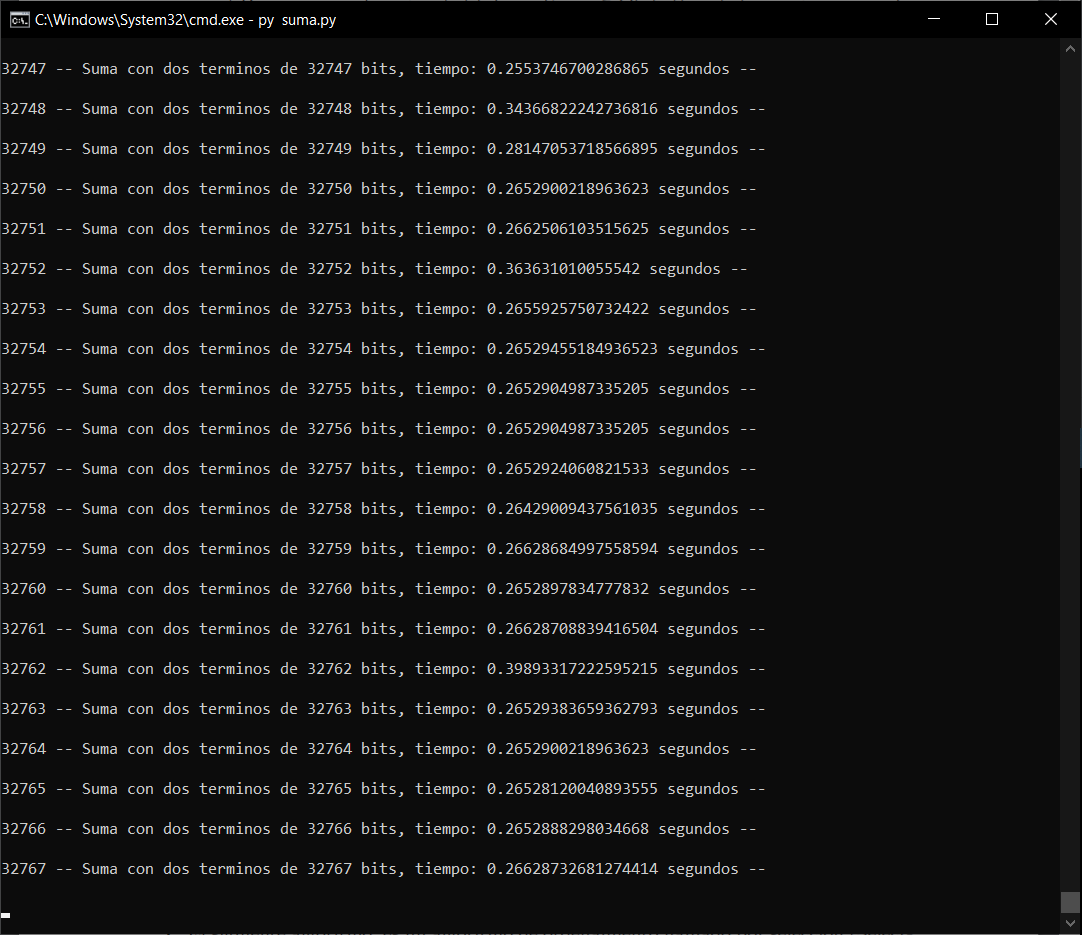
\includegraphics[height = 7.5cm]{c4}
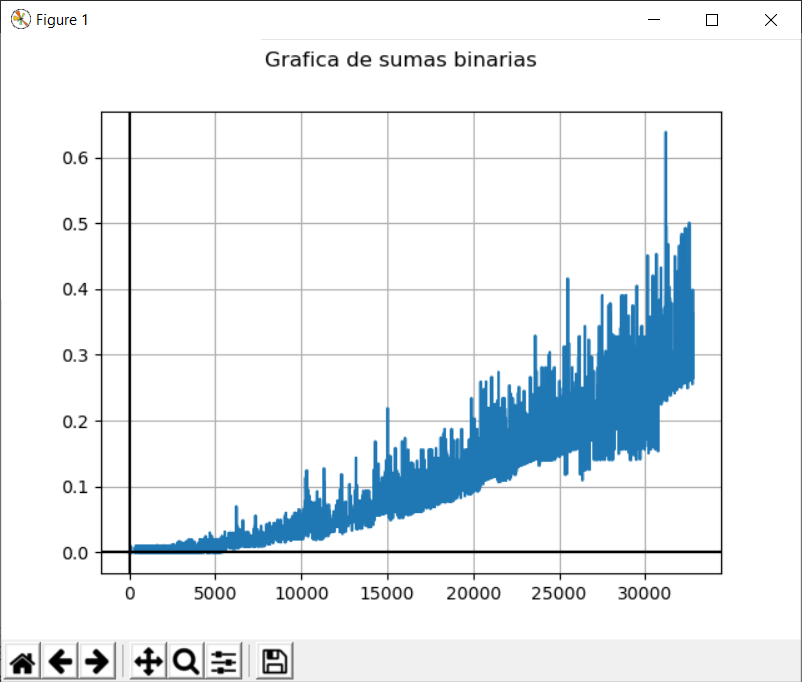
\includegraphics[height = 7.5cm]{g4}
\end{center}
Y se repiti\'o el experimento con potencias de 2, primero se muestra con \texorpdfstring{2\textsuperscript{21}}{2 21} bits con un tiempo tardado de 17 minutos aproximadamente
\begin{center}
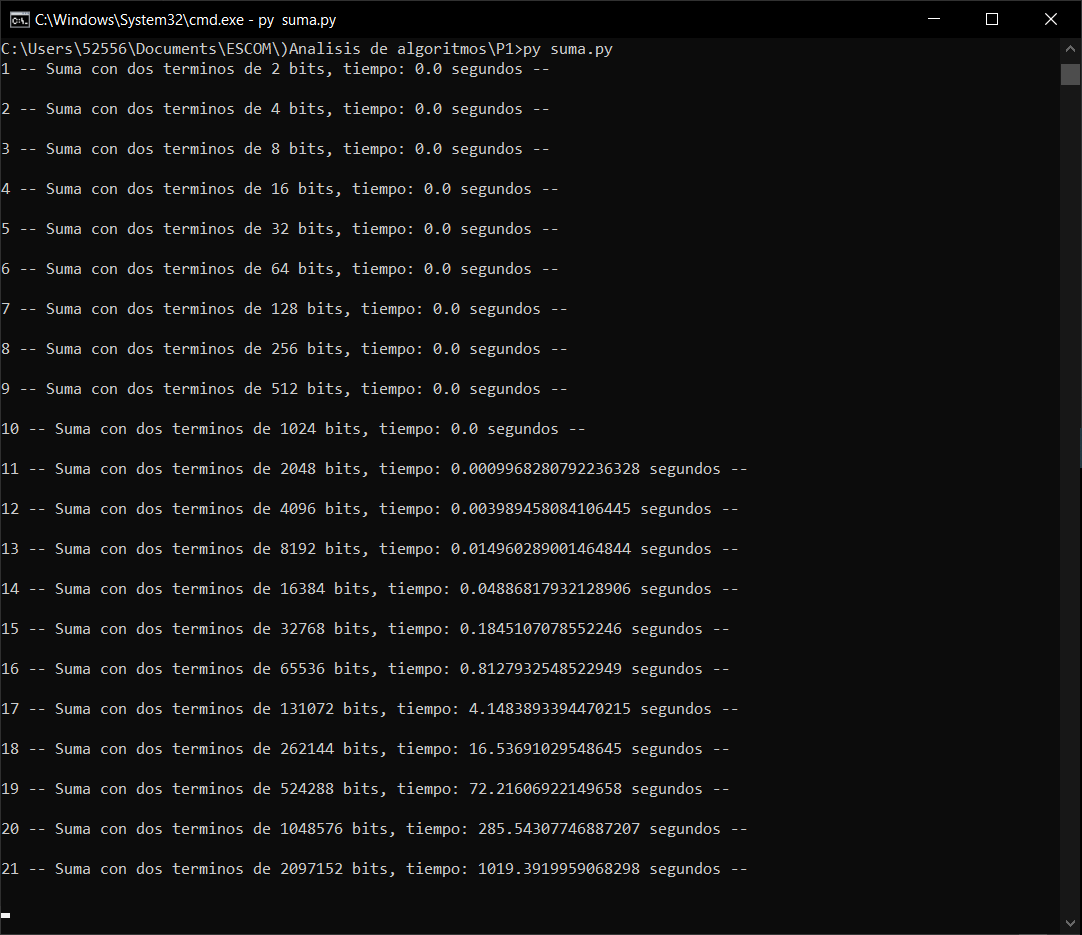
\includegraphics[height = 7.5cm]{c2}
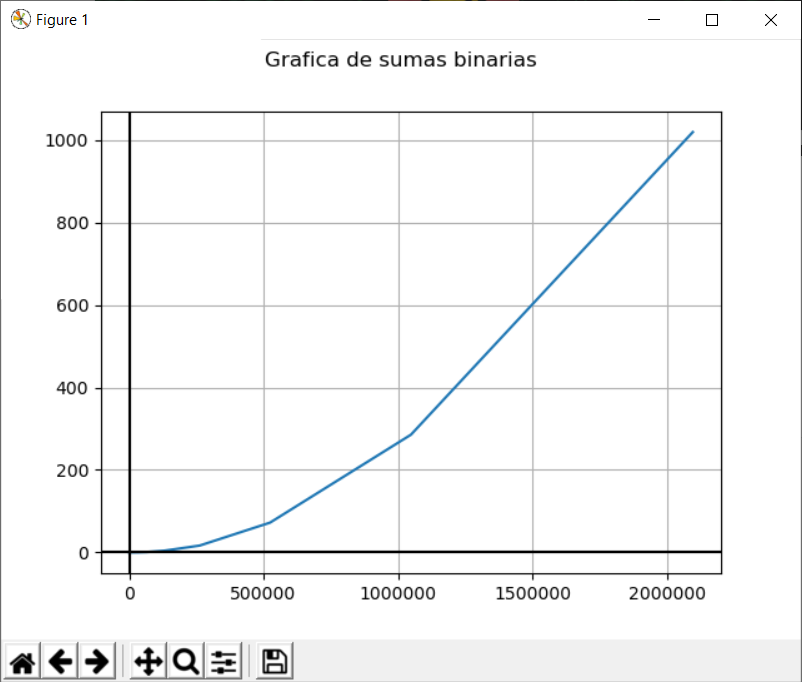
\includegraphics[height = 7.5cm]{g2}
\end{center}
Y por \'ultimo se muestra con \texorpdfstring{2\textsuperscript{23}}{2 23} bits, donde los \'ultimos puntos de la gr\'afica se vieron un poco afectados por la computadora 
que estuvo realizando otras tareas, ya que para este proceso se tardo en ejecutar un aproximado de 5 horas y media
\begin{center}
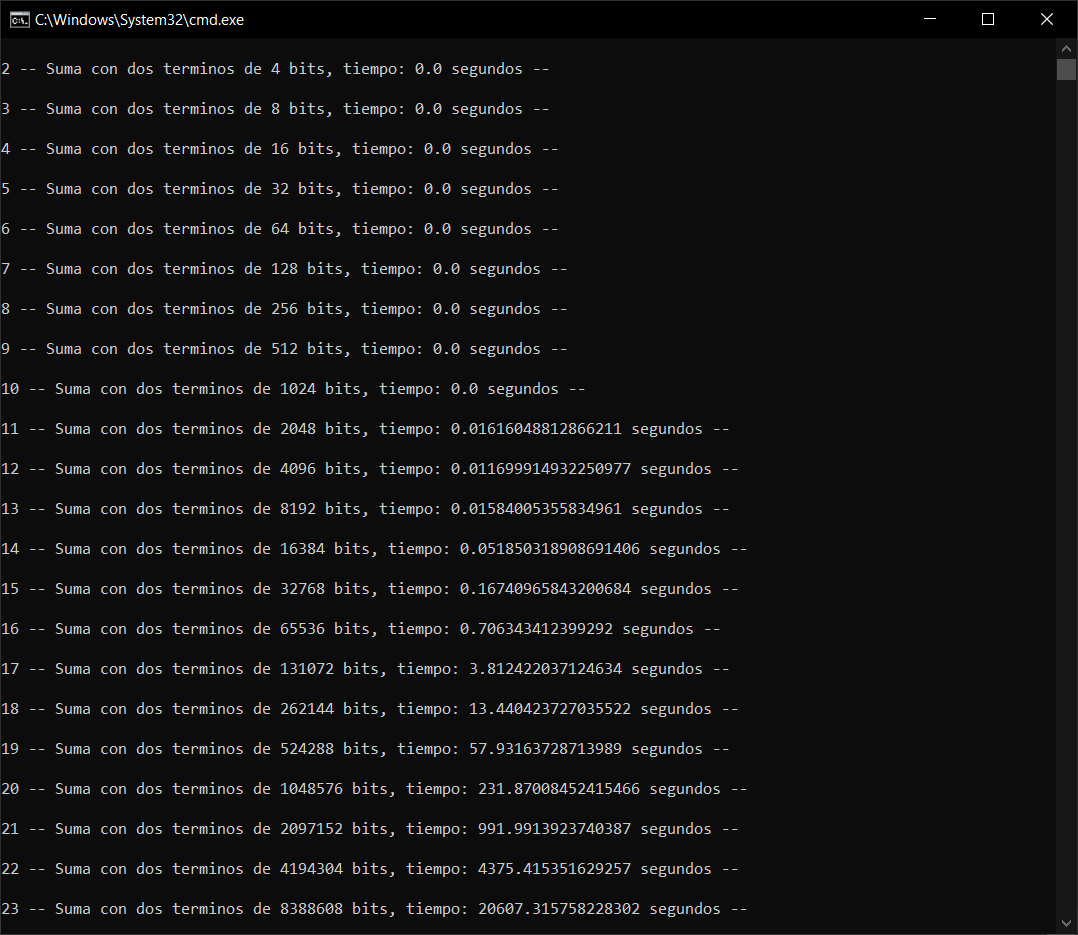
\includegraphics[height = 7.5cm]{c3}
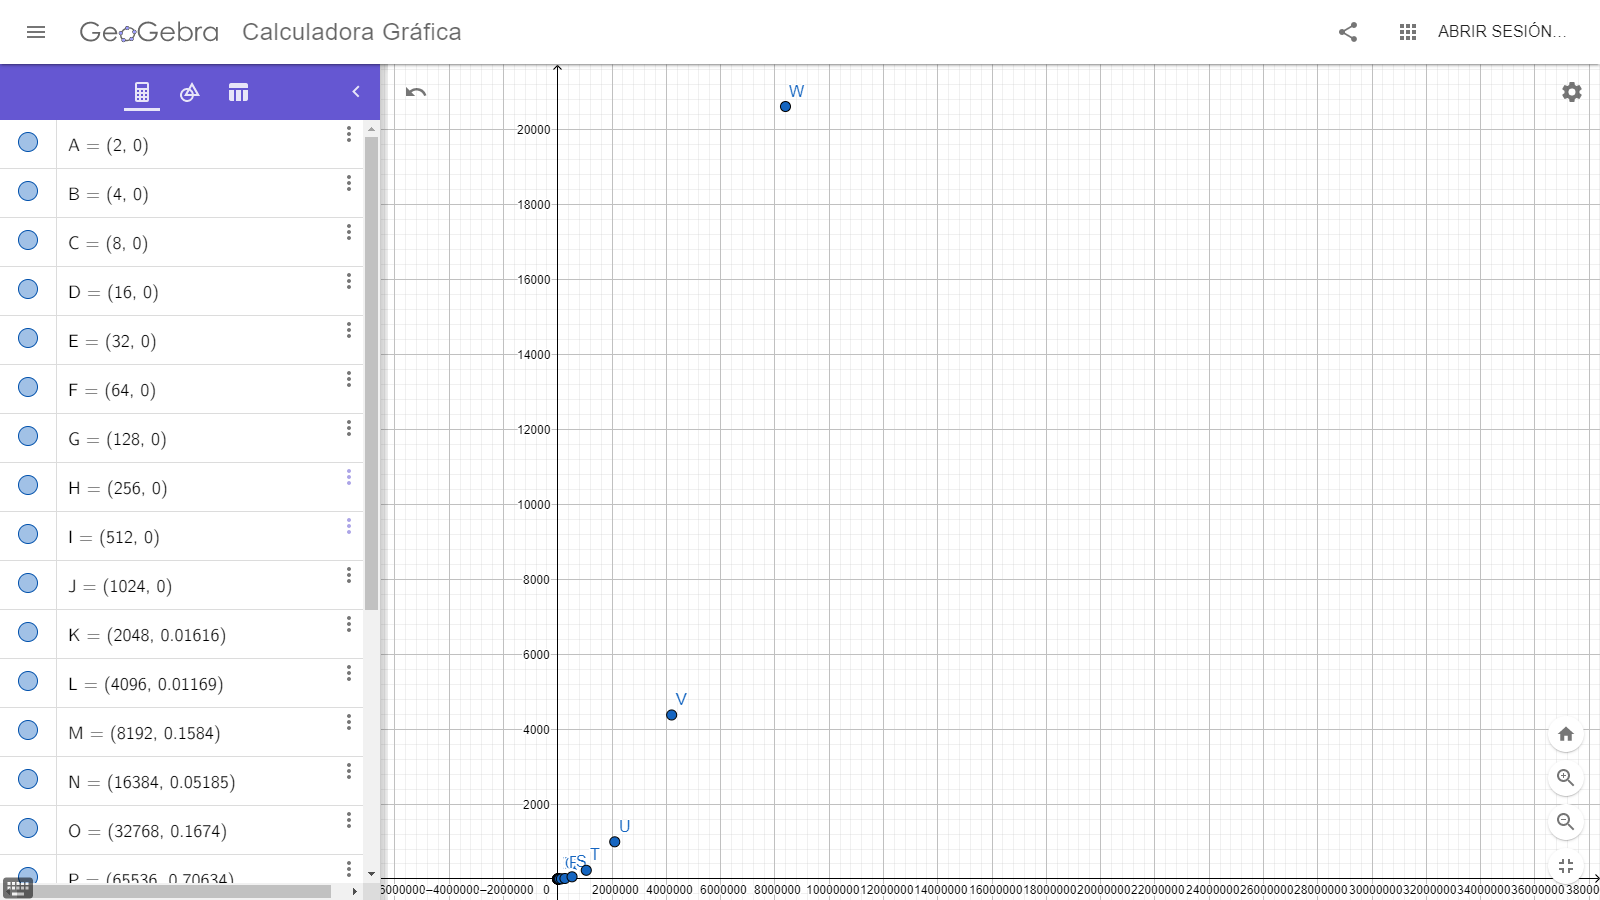
\includegraphics[height = 7.5cm]{g3}
\end{center}
Para proponer una función $O(g(n))$ observamos que si se realiza esta prueba en otra computadora, los tiempos pueden variar muy poco
\begin{center}
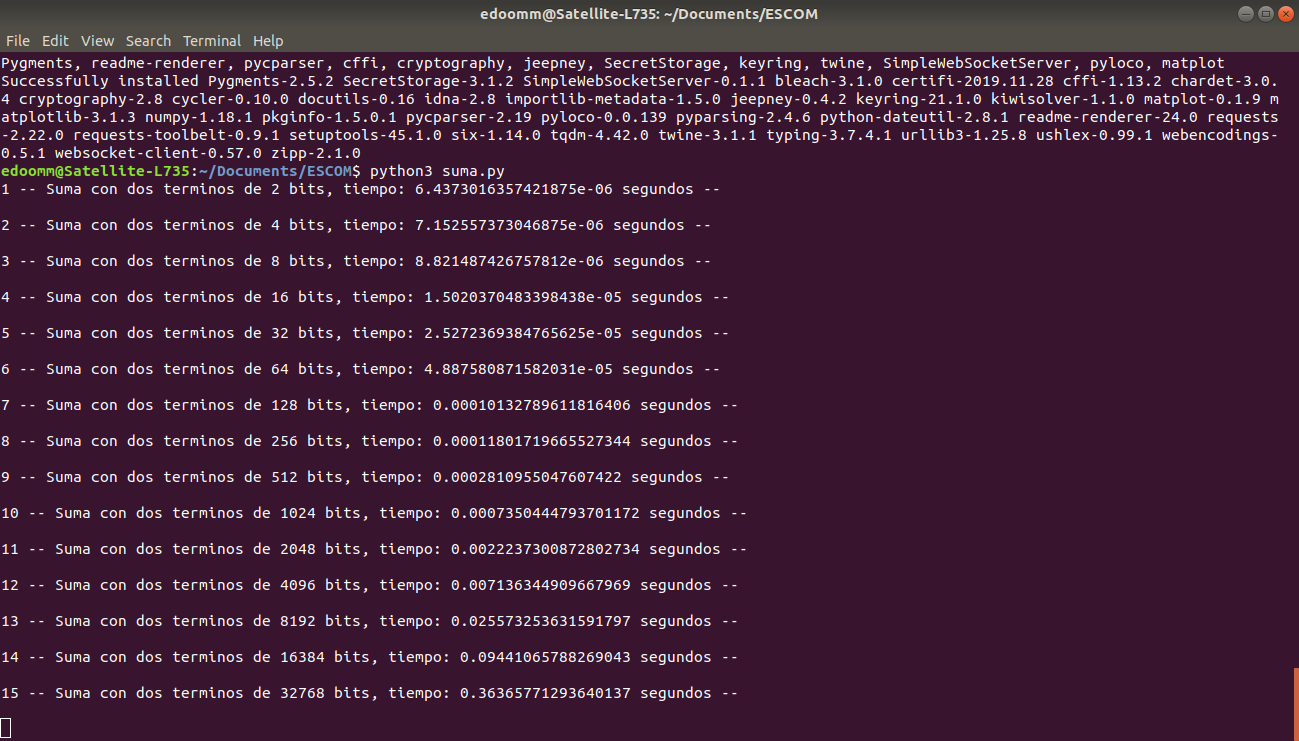
\includegraphics[height = 7.5cm]{c5}
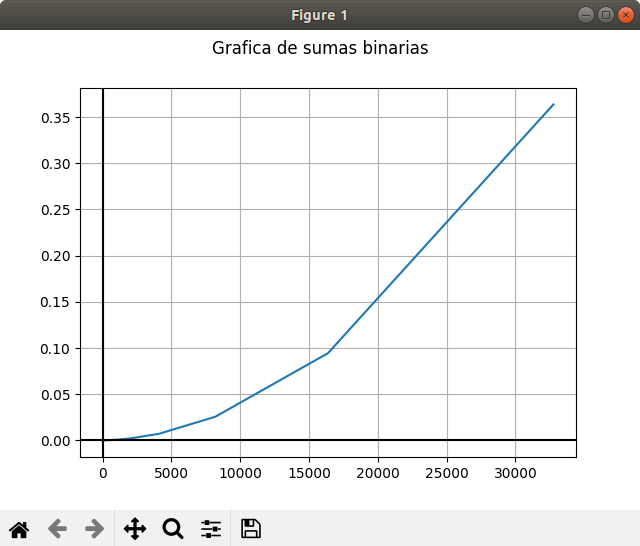
\includegraphics[height = 7.5cm]{g5}
\end{center}
Por lo tanto, si este algoritmo es analizado a priori, podemos observar que tendra $O(n)$, esto de igual forma 
se verifica con el analisis a posteriori realizado en la practica y lo podemos ver claramente en la siguiente gráfica
\begin{center}
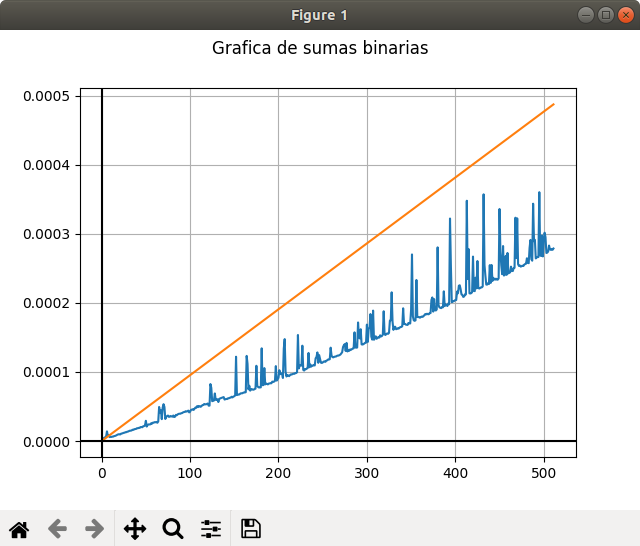
\includegraphics[height = 7.5cm]{g6}
\end{center}
Así también, se puede acotar por otra función \texorpdfstring{c\textsubscript{1}}{c 1}$g(n)$, pero en la notación $O$ los coeficientes pueden ser omitidos 
Así bien,
\[Suma \in O(n)\]

\subsection{M\'inimo com\'un divisor mediante algoritmo de Euclides}
Al ingresar un par de números enteros positivos (`m' y `n'), se evalúan mediante el algoritmo de Euclídes (descrito anteriormente), y se muestra al usuario en pantalla el mínimo común divisor. A continuación se presenta el algoritmo de Euclides 
implementado en Python 
\begin{lstlisting}
	Euclides (M[1, ..., n], N[1, ..., n])					
							
	while n!=0 do					
		
		r <- m mod n 				
					
		m <- n 					
		
		n <- r 					
	
	return m

mcd = Euclides(m, n)					
\end{lstlisting}

Para obtener el mcd tambien se implemento el algoritmo para desarrollar la Serie de Fibonacci, el cual es el siguiente:
\begin{lstlisting}
    Fibonacci (M[1, ..., n], N[1, ..., n])
        m, n <- 0,1
        
        while m < o do
        
            m, n <- n, m+n
\end{lstlisting}
Se realizaron pruebas de escritorio implementadas en python las cuales se muestran a continuación con numeros aleatorios para determinar el tamaño de la serie de Fibonacci. 
En la siguiente pantalla se muestra una prueba con una cantidad menor a 10,000, mostrando la serie hasta el numero más cercano al seleccionado y se saca el mcd de los 2 numeros siguientes al ultimo junto con el tiempo de ejecución.
\begin{center}
    \includegraphics[width=1.0\textwidth]{eu1.png}
\end{center}
Al observar los primeros resultados y cambiar el limite de la serie para observar su tiempo de ejecucion, continuamos 
a trabajar con el i-esimo número de la serie de fibonacci, el cual nos representa el peor caso en el algoritmo de Euclides. A continuacion se muestra el tiempo de ejecución de ejecucion que tarda en realizarce cada operacion, el ejemplo se muestra con 70.
\begin{center}
    \includegraphics[width=1.0\textwidth]{eu2.png}
\end{center}
La grafica de estos tiempo quedo de la siguiente manera 
\begin{center}
    \includegraphics[width=1.0\textwidth]{eu3.png}
\end{center}
\section{Anexo}
\subsection{Select-Sort}
\textbf{Select-Sort(A[0, . . . , 4 - 1])} \hspace*{1cm}Se recibe un
arreglo de 4 elementos \newline
Iteración 1:\newline
for j $\longleftarrow$ 0 to j $\leq$ n - 2 do \hspace*{1cm}Para j=0
hasta j$\leq$(4-2) \newline
\hspace*{1cm}k $\longleftarrow$ j \hspace*{1cm}La variable k toma el
valor de 0 \newline
\hspace*{1cm}for i $\longleftarrow$ j + 1 to i $\leq$ n - 1 do
\hspace*{1cm}Para i= 0 + 1 hasta i$\leq$ 4 - 1 \newline
\hspace*{1.5cm}if A[i] < A[k] then \hspace*{1cm}Si A[1] < A[0]
\newline
\hspace*{2cm}k $\longleftarrow$ i \hspace*{1cm}La variable k, se le
asigna el valor de i=1 \newline
\hspace*{1.5cm}Intercambia (A[j],A[k]) \hspace*{1cm}Se coloca el
contenido de A[0] A[1]\newline \newline
Iteración 2:\newline
for j $\longleftarrow$ 0 to j $\leq$ n - 2 do \hspace*{1cm}Para j=1
hasta j$\leq$(4-2) \newline
\hspace*{1cm}k $\longleftarrow$ j \hspace*{1cm}La variable k toma el
valor de 1 \newline
\hspace*{1cm}for i $\longleftarrow$ j + 1 to i $\leq$ n - 1 do
\hspace*{1cm}Para i= 1 + 1 hasta i$\leq$ 4 - 1 \newline
\hspace*{1.5cm}if A[i] < A[k] then \hspace*{1cm}Si A[2] < A[1]
\newline
\hspace*{2cm}k $\longleftarrow$ i \hspace*{1cm}La variable k, se le
asigna el valor de i=2 \newline
\hspace*{1.5cm}Intercambia (A[j],A[k]) \hspace*{1cm}Se coloca el
contenido de A[1] A[2]\newline \newline
Iteración 3:\newline
for j $\longleftarrow$ 0 to j $\leq$ n - 2 do \hspace*{1cm}Para j=2
hasta j$\leq$(4-2) \newline
\hspace*{1cm}k $\longleftarrow$ j \hspace*{1cm}La variable k toma el
valor de 2 \newline
\hspace*{1cm}for i $\longleftarrow$ j + 1 to i $\leq$ n - 1 do
\hspace*{1cm}Para i= 2 + 1 hasta i$\leq$ 4 - 1 \newline
\hspace*{1.5cm}if A[i] < A[k] then \hspace*{1cm}Si A[3] < A[2]
\newline
\hspace*{2cm}k $\longleftarrow$ i \hspace*{1cm}La variable k, se le
asigna el valor de i=3 \newline
\hspace*{1.5cm}Intercambia (A[j],A[k]) \hspace*{1cm}Se coloca el
contenido de A[2] A[3]
\subsubsection{Pruebas de escritorio}
Para este algoritmo el código final implementando en Python quedó conformado de la siguiente forma
\begin{lstlisting}
def selectSort(A):
    j = 0
    while j <= len(A) - 2:
        k = j
        i = j + 1
        while i <= len(A) - 1:
            if A[i] < A[k]:
                k = i
            i += 1
        A[j], A[k] = A[k], A[j]
        j += 1

    print(A)
\end{lstlisting}
Y a continuación se muestran algunas pruebas con arreglos de tamaño 10, con elementos del 0 al 10
\begin{center}
    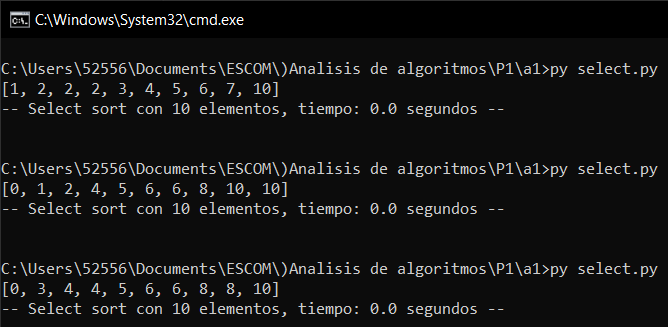
\includegraphics[height = 6.5cm]{pruebaa1.png}
\end{center}
\subsubsection{Cálculo del orden de complejidad en el peor de los
casos}
Procedemos a reescribir las líneas de código y calcular sus costos
en una tabla debajo de éstas.\newline \newline
\textbf{Select-Sort(A[0, . . . , 4 - 1])} \hspace*{1cm}Se recibe un arreglo de 4 elementos \newline
for j $\longleftarrow$ 0 to j $\leq$ n - 2 do\newline
\hspace*{1cm}k $\longleftarrow$ j\newline
\hspace*{1cm}for i $\longleftarrow$ j + 1 to i $\leq$ n - 1 do
\newline
\hspace*{1.5cm}if A[i] < A[k] then\newline
\hspace*{2cm}k $\longleftarrow$ i\newline
\hspace*{1.5cm}Intercambia (A[j],A[k])\newline \newline
\begin{tabular}{|l|l|}
\hline
Línea & Costo\\
\hline
$C_{1}$ &n\\
\hline
$C_{2}$ &n-1\\
\hline
$C_{3}$ & $\Sigma_{i=1}^{n}t_{i}$ \\
\hline
$C_{4}$ & $\Sigma_{i=1}^{n}t_{i}-1$ \\
\hline
$C_{5}$ & n-1 \\
\hline
\end{tabular}
\\ \\
$T_{(n)} = C_{1}n+(n-1)(C_{2}+C_{5})+C_{3}(\Sigma_{i=1}
^{n}t_{i})+C_{4}(\Sigma_{i=1}^{n}t_{i}-1)$ \newline
$T_{(n)} = C_{1}n+(n-1)(C_{2}+C_{5})+C_{3}(\Sigma_{i=1}^{n}n_{i})
+C_{4}(\Sigma_{i=1}^{n}n_{i}-1)$ \newline
$T_{(n)} = (C_{3}+C_{4})n^{2}+(C_{5}-C_{4}+C_{2}+C_{1})n-C_{5}-C_{2}
$ \newline
$\therefore T_{(n)}\in\bigcirc_{(n^{2})}$
\subsection{Máximo de un arreglo}
\subsubsection{Prueba de escritorio}
Nuestro algoritmo quedó implementado como se muestra a continuación.
\begin{lstlisting}
Maximo (A[0, 1, ... n-1])
    max = A[0]
    for i <- 0 to i < n do
        if A[i] > max then
            max <- A[i]
\end{lstlisting}
Y en seguida se muestran 4 pruebas que se hicieron con arreglos de tamaño 10, con 
elementos que van del 0 al 10
\begin{center}
    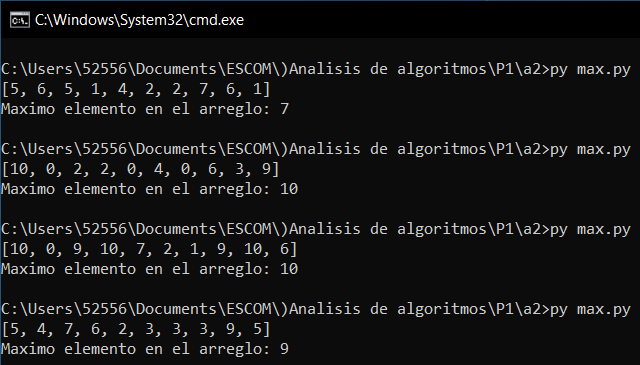
\includegraphics[height = 6cm]{maximocons.png}
\end{center}
\subsubsection{Cálculo del orden de complejidad en el peor de los casos}
\subsection{Problema 8 del problemario}
Para la primera parte se tuvo el siguiente algoritmo
\begin{lstlisting}
Algoritmo1 (a[0, ..., n-1])
    for i=n-1 to i>0 do
        for j=0 to j<i
            if a[j]>a[j+1] then
                temp=a[j]
                a[j]=a[j+1]
                a[j+1]=temp
\end{lstlisting}
Asi pues, para calcular el orden de complejidad, analizamos linea por linea este
algoritmo.
\begin{center}
\begin{tabular}{|l|l|}
\hline
Línea & Costo\\
\hline
$C_{1}$ &n\\
\hline
$C_{2}$ & $\Sigma_{i=1}^{n-1}t_{i}$\\
\hline
$C_{3}$ & $\Sigma_{i=1}^{n-1}(t_{i}-1)$ \\
\hline
$C_{4}$ & $\Sigma_{i=1}^{n-1}(t_{i}-1)$ \\
\hline
$C_{5}$ & $\Sigma_{i=1}^{n-1}(t_{i}-1)$ \\
\hline
$C_{6}$ & $\Sigma_{i=1}^{n-1}(t_{i}-1)$ \\
\hline
\end{tabular}
\end{center}
Asi pues, notamos que en el mejor de los casos, el algoritmo no ejecuta el cuerpo del if , y en el peor caso, ejecuta el cuerpo del if. Podemos notar que las sentencias dentro del cuerpo del if son $O(1)$.
Luego entonces, se tiene.
\begin{center}
\begin{tabular}{|l|l|}
\hline
i & ti\\
\hline
1 & n\\
\hline
2 & n-1\\
\hline
... & ...\\
\hline
n & n-i+1\\
\hline
\end{tabular}
\end{center}
Luego,
\begin{center}
T(n) = $C_{1}$n + $C_{2}\Sigma_{i=1}^{n-1}(n-i+1)$\ + $C_{3}\Sigma_{i=1}^{n-1}(n-i)$ \ + $C_{4}\Sigma_{i=1}^{n-1}(n-i)$ \ + $C_{5}\Sigma_{i=1}^{n-1}(n-i)$ \ + $C_{6}\Sigma_{i=1}^{n-1}(n-i)$ \\
\end{center}
Después,
\begin{center}
T(n) = $C_{1}$n + $C_{2}\Sigma_{i=1}^{n-1}n$ - $C_{2}\Sigma_{i=1}^{n-1}i$ +
$C_{2}\Sigma_{i=1}^{n-1}1$ + $C_{3}\Sigma_{i=1}^{n-1}n$ - $C_{3}\Sigma_{i=1}^{n-1}i$ + $C_{4}\Sigma_{i=1}^{n-1}n$ - $C_{4}\Sigma_{i=1}^{n-1}i$ + $C_{5}\Sigma_{i=1}^{n-1}n$ - $C_{5}\Sigma_{i=1}^{n-1}i$ + $C_{6}\Sigma_{i=1}^{n-1}n$ - $C_{6}\Sigma_{i=1}^{n-1}i$ \\
\end{center}
Es decir,
\begin{center}
T(n) = $C_{1}$n + $(C_{2} + C_{3} + C_{4} + C_{5} + C_{6})(n^{2} - n)$ - $(C_{2} + C_{3} + C_{4} + C_{5} + C_{6})\frac{n^{2}-n}{2} + C_{2}(n - 1)$ \\
\end{center}
Por lo tanto,
\begin{center}
T(n) = $\frac{1}{2}(C_{2} + C_{3} + C_{4} + C_{5} + C_{6})(n^{2}-n) + (C_{1} + C_{2})n - C_{2}$
\end{center}
Así podemos observar que $T(n)$ es de la forma,
\begin{center}
T(n) = $a + bn + cn^{2}$
\end{center}
\begin{center}
$\therefore T_{(n)}\in O{(n^{2})}$
\end{center}
\subsection{Máquinas de Turing}
Para la primer máquina de Turing se tuvo que implementar una máquina capaz de sacar el complemento de un número binario, es decir, convertir los 1 en 0.
\begin{tikzpicture}[shorten >=1pt,node distance=4cm,on grid,auto]
\node[state, initial] (0) {$q_0$};
\node[state, accepting] (1) [right=of 0] {$q_1$};
    \path[->]
    (0) edge                    node {$B\:/B,\:R$} (1)
    (0) edge [loop above]       node {$0\:/1,\:R$} (0)
    (0) edge [loop below]       node {$1\:/0,\:R$} (0)
\end{tikzpicture}
\newline
\newline
La siguiente máquina de Turing pedida fue una capaz de realizar sumas binarias y quedo implementada como se muestra a continuación.

\section{Conclusiones}
Las conclusiones de manera general y de manera individual. En lo general, podr\'ian escribir,
errores que se presentaron y como se resolvieron, podr\'ian escribir observaciones de como
mejorar el algoritmo, si quedaron los resultados esperados o no, y por que, etc.
Las conclusiones individuales ya cada quien sabr\'a que redactar. A las conclusiones individuales
se les anexar\'a una fotografía del cada alumno.
Conclusiones Alumno 1 (FOTO)
Conclusiones ALumno 2 (FOTO)
\section{Bibliograf\'ia}
Mostrar referencias en formato IEEE.
\end{document}